 
\chapter{Branch Prediction}\label{chapter:bpd}

This chapter discusses how BOOM predicts and resolves branch predictions.

BOOM uses two levels of branch prediction- a single-cycle ``next-line predictor" (NLP), and a slower but more complex ``backing predictor" (BPD).\footnote{Unfortunately, the terminology in the literature gets a bit muddled here in what to call different types and levels of branch predictor. I have seen ``micro-BTB" versus ``BTB", ``NLP" versus ``BHT", and ``cache-line predictor" versus ``overriding predictor". 
Although the Rocket code calls its own predictor the ``BTB", I have chosen to refer to it in documentation as the ``next-line predictor", to denote that it is a combinational predictor that provides single-cycle predictions for fetching ``the next line", and the Rocket BTB encompasses far more complexity than just a ``branch target buffer" structure.  Likewise, I have chosen the name ``backing predictor" as I believe it is the most accurate name, while simultaneously avoiding being overly descriptive of the internal design (is it a simple BHT? Is it tagged? Does it override the NLP?).
{\color{red} But in short, I am open to better names!}}



\begin{figure}[ht]
	\centering
	\centerline{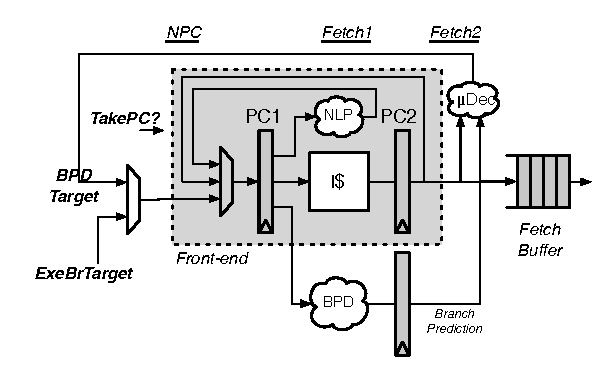
\includegraphics[scale =1] {figures/frontend}}
	\caption{ \small The Fetch Unit.}
	\label{fig:fetch}
\end{figure}


\section{The Rocket Next-line Predictor (NLP)}

BOOM instantiates the Rocket core's Front-End, which fetches instructions and predicts every cycle where to fetch the next instructions. If a misprediction is detected in BOOM's backend, or BOOM's own backing predictor wants to redirect the pipeline in a different direction, a request is sent to the Front-End and it begins fetching along a new instruction path. 

The next-line predictor (NLP) takes in the current PC being used to fetch instructions (the {\em Fetch PC}) and predicts combinationally where the next instructions should be fetched for the next cycle. If predicted correctly, there are no pipeline bubbles. 

The next-line predictor is an amalgamation of a fully-associative branch target buffer (BTB), a {\em gshare} branch history table (BHT), and a return address stack (RAS) which work together to make a fast, but reasonably accurate prediction.

\subsection{NLP Predictions}

The {\em Fetch PC} first performs a tag match to find a uniquely matching BTB entry.  
If a hit occurs, the BTB entry will make a prediction in concert with the BHT and RAS as to whether there is a branch, jump, or return found in the {\em fetch packet} and which instruction in the {\em fetch packet} is to blame.  
The BTB entry also contains a predicted PC target, which is used as the {\em Fetch PC} on the next cycle.

\TODO{add an image showing how the BTB stores data, and makes predictions}




The hysteresis bits (governed by a {\em gshare} predictor) are only used on a BTB entry {\em hit} and if the predicting instruction is a branch. 

If the BTB entry contains a {\em return} instruction, the RAS stack is used to provide the predicted return PC as the next {\em Fetch PC}. The actual RAS management is governed externally. 

For area-efficiency, the high-order bits of the PC tags and PC targets are stored in a compressed file.


\subsection{NLP Updates}

Each branch passed down the pipeline remembers not only its own PC, but also its {\em Fetch PC} (the PC of the head instruction of its {\em fetch packet}).\footnote{In reality, only the very lowest bits must be saved, as the higher-order bits will be the same.}  Upon Branch Resolution, the NLP is updated with the outcome of the branch.  

When the NLP makes a prediction, it is actually using the BTB to tag match against the predicted branch's {\em Fetch PC}, and not the PC of the branch itself.  
The NLP must predict across the entire {\em fetch packet} which of the many possible branches will be the dominating branch that redirects the PC.  
For this reason, we use a given branch's {\em Fetch PC} rather than its own PC in the BTB tag match. %Even for superscalar fetching, only a single {\em Fetch PC} is passed to the NLP. 
\footnote{Each BTB entry corresponds to a single {\em Fetch PC}, but it is helping to predict across an entire {\em fetch packet}. However, the BTB entry can only store meta-data and target-data on a single control-flow instruction.  While there are certainly pathological cases that can harm performance with this design, the assumption is that there is a correlation between which branch in a {\em fetch packet} is the dominating branch relative to the {\em Fetch PC}, and - at least for narrow fetch designs - evaluations of this design has shown it is very complexity-friendly with no noticeable loss in performance. Some other designs instead choose to provide a whole bank of BTBs for each possible instruction in the {\em fetch packet}.} 





\section{The Backing Predictor}

\TODO{...}

\section{Branch Prediction Configurations}

There are a number of parameters provided to govern the branch prediction in BOOM.

\TODO{...}
 
